\documentclass[ignorenonframetext,hyperref={pdftex,unicode}]{beamer}

\usetheme{Epam}

% Каб дадаваць зыходны код
\usepackage{listings}
% Дазволіць устаўляць LaTeX код паміж значкамі
\lstset{escapeinside=||}

\usepackage{indentfirst,amsfonts} % падтрымка кірылічных тыпаграфічных стандартаў

\usepackage[english,russian]{babel}
\usepackage[T2A]{fontenc}
\usepackage[utf8]{inputenc}

% for hyperlinks
\usepackage{hyperref}
% for strike-out text
\usepackage[normalem]{ulem}

\ifpdf
        \usepackage{cmap} % пошук па PDF
        \pdfcompresslevel=9 % узровень кампрэсіі PDF
\else
        \usepackage{graphicx}
\fi

% Слайд "Пытанні"
\newcommand{\questionslide} {
	\vfill
	\begin{beamercolorbox}[rounded=true,shadow=true,sep=8pt,center]{title}
		\huge\bf Пытанні? \par
		\vskip0.25em
	\end{beamercolorbox}
	\begin{beamercolorbox}[sep=8pt,center]{foot1} 
		\insertauthor\par
	\end{beamercolorbox}
}


\title{Досвед апацоўкі відэа з дапамогай kdenlive}
\author[Андрэй Захарэвіч]{Андрэй Захарэвіч\\ andrej\_zacharevicz@epam.com}


\begin{document}

\frame{\titlepage} 


\section{Што мелі ад пачатку} 

\begin{frame}{З чаго пачыналі} 
	Як і ўсе, напачатку мы здымалі адной камерай і слайды, і дакладчыка. Атрымлівалася ад недобра да жудасна.

	Звычайна мы добра бачым альбо дакладчыка (што часта не самае галоўнае), альбо слайды.
	\begin{center}
 		
\includegraphics[height=0.5\textheight,keepaspectratio]{1}		
	\end{center}
\end{frame}

\section{Што хацелі атрымаць} 

\begin{frame}{Куды мы мусім рухацца} 
	Слайды мусяць фіксавацца асобна і займаць большую частку плошчы кадра. Ідэю я сустракаў і раней, але канчаткова зразумеў, крыху пазнаёміўшыся з матэрыяламі пра Seminar Assembler[1][2] Стаса Фаміна
	\begin{center}
 		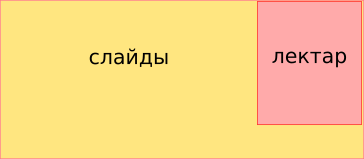
\includegraphics[height=0.5\textheight,keepaspectratio]{2}		
	\end{center}
\end{frame}

\begin{frame}{Што яшчэ} 
	Але гэта галоўная ідэя і па факце слайд можна дапаўняць шэрагам іншых аб'ектаў і відэафайлаў, якія не з'яўляюцца абавязковымі, але паляпшаюць уражанне ад відэа.
	\begin{center}
 		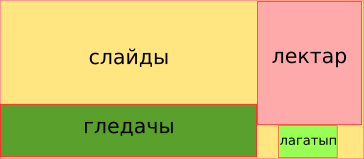
\includegraphics[height=0.5\textheight,keepaspectratio]{3}		
	\end{center}
\end{frame}

\section{Што атрымалася}

\begin{frame}[fragile]
	\frametitle{Чым карысталіся} 
	Для таго каб здзейсніць постапрацоўку матэрыялаў дакладу я карыстаўся наступнымі пакетамі:
	\begin{itemize}
		\item kdenlive[3]
		\item скрыпт для захопу скрынкаста з дапамогай ffmpeg[4]
		\item pdftoppm[5] з пакету Poppler[6] (poppler-utils у Debian)
	\end{itemize}
	
	Прыклад ужывання pdftoppm:
		\begin{lstlisting}[language=bash]
pdftoppm -jpeg slides.pdf prefix
		\end{lstlisting}
\end{frame}

\frame{\questionslide}

\begin{frame}{Спіс літаратуры і спасылкі}
	\begin{thebibliography}{10}
	\beamertemplatetextbibitems
	\bibitem{}
		{\sc \href{http://wiki.4intra.net/SeminarAssembler}{SeminarAssembler}};
	\bibitem{}
		{\sc \href{https://abf.io/belonesox/seminar-assembler/}{Зыходнікі SeminarAssembler}};
	\bibitem{}
		{\sc \href{https://kdenlive.org/}{Kdenlive}};
	\bibitem{}
		{\sc \href{https://github.com/measles/mlug\_screencast\_sound}{Скрыпт для запісу скрынкастаў}};
	\bibitem{}
		{\sc \href{http://linux.die.net/man/1/pdftoppm}{pdftoppm}};
	\bibitem{}
		{\sc \href{https://poppler.freedesktop.org/}{Афіцыйная старонка Poppler}};
	\end{thebibliography}
\end{frame}

\end{document}
